\section{Methods}\label{sec:methods}

\textbf{Retinal recordings.}
Since I don't realize any experiments myself, I will try here to give as few
details
as necessary for the understanding of the rest of the work. Still, experimental
recording of the retina is a very interesting topic and the reader can look
here for more information. % Useful ?
The laboratory has access to three experimental rooms that enable
state-of-the-art experimentation
on the retina.	For this project, we record the activity of retinal ganglion
cells
using a multi-electrode array. The retina is placed on a ???
% TO COMPLETE

% A part to complete

\textbf{Stimuli design.}
The stimuli used in this project are composed of two images, one synthetic
adaptation image followed by a natural image. Adaptation images are taken from
a pull of three different patterns: a grey screen used as control, a
checkerboard of X*X checks and the same checkerboard with inverted colors (Fig.
TO ADD). Natural images are taken from ADD REFERENCE. XXXX images were used for
training the CNN, 10 were used to test the CNN and among them, 3 were used to
record an estimation of the LSTA of each cell.
Adaptation and natural images are always paired together to form a single
stimulus pair, also referenced as a clip. Each frame is XXXxXXX pixels wide and
each clip is 2*400ms long.

% Give details about how the images are built for the camera?

The training set is composed of XXXX clips, each composed of the grey
adaptation image followed by a natural image. The test set is composed of 30
clips, each repeated 30 times. The test clips are composed 10 different natural
images preceded by each adaptation (3 different clips for each natural image).
The dataset used to record LSTA is composed of 9 different clips repeated 1000
times. Each clip is composed of one of the three selected natural images
preceded by one of the adaptation patterns.

We first used 4 different natural images while computing the LSTA of each cell,
each 12 different clips being repeated 12 times. We found that the estimation of the LSTA was too unstable with only 750 repetitions. In following experiments we excluded the image that yielded the least amount of stable estimations of LSTA (20\% average success rate as compared to 42\% average success rate for the other three images). We then used 3 different natural images while computing the LSTA of each cell, each 9 different clips being repeated 1000 times. We found that the estimation of the LSTA was stable with 1000 repetitions.

\tab\textbf{Data processing.}
Multi-electrode array experimental data, including semi-automatized spike sorting and cell typing.
This process can take up to an entire day for a single experiment. I am also
able to share my programming skill to help and improve the data pipeline of the
laboratory. This part of my project includes design of experimental stimulus,
trustworthy sanity checks and high quality data visualization.

\textbf{Modeling.} This should be the main part of my internship and also the
most challenging. We are designing a dynamical model of the retinal fast
adaptation. In fact, we mostly look at the evolution of the response from an
image to another, meaning that the dynamic we observe only spans two points in
time. This reduction makes the model more realistic to study. Most of this job
can be summarized as model design, python programming, sensitivity analysis and
data fitting. By comparing how different modeling strategies reproduce the
observed LSTA in the data, we can gain insight on how fast adaptation to
natural scene is implemented in the retina.
%I think what is missing here is what question you want to answer with this. We should discuss this more. 

Our baseline model is the LNLN model of ganglion cell widely used in the
literature. Each neuron is encoded as a spatial linear filter chained with a
non-linearity (usually an activation linearity in the like of ReLU). A single
layer of subunit neurons, representing bipolar cells, converge into a single
modeled ganglion cell.	We would like to add temporal dynamics to this model,
either by adding a time dimension to the spatial liner filter of the cells or
by considering a gain control mechanism. This last mechanism consists in
scaling up or down the present output depending on past outputs (Figure
TO FIND~\cite{}).

\begin{figure}
    \centering
    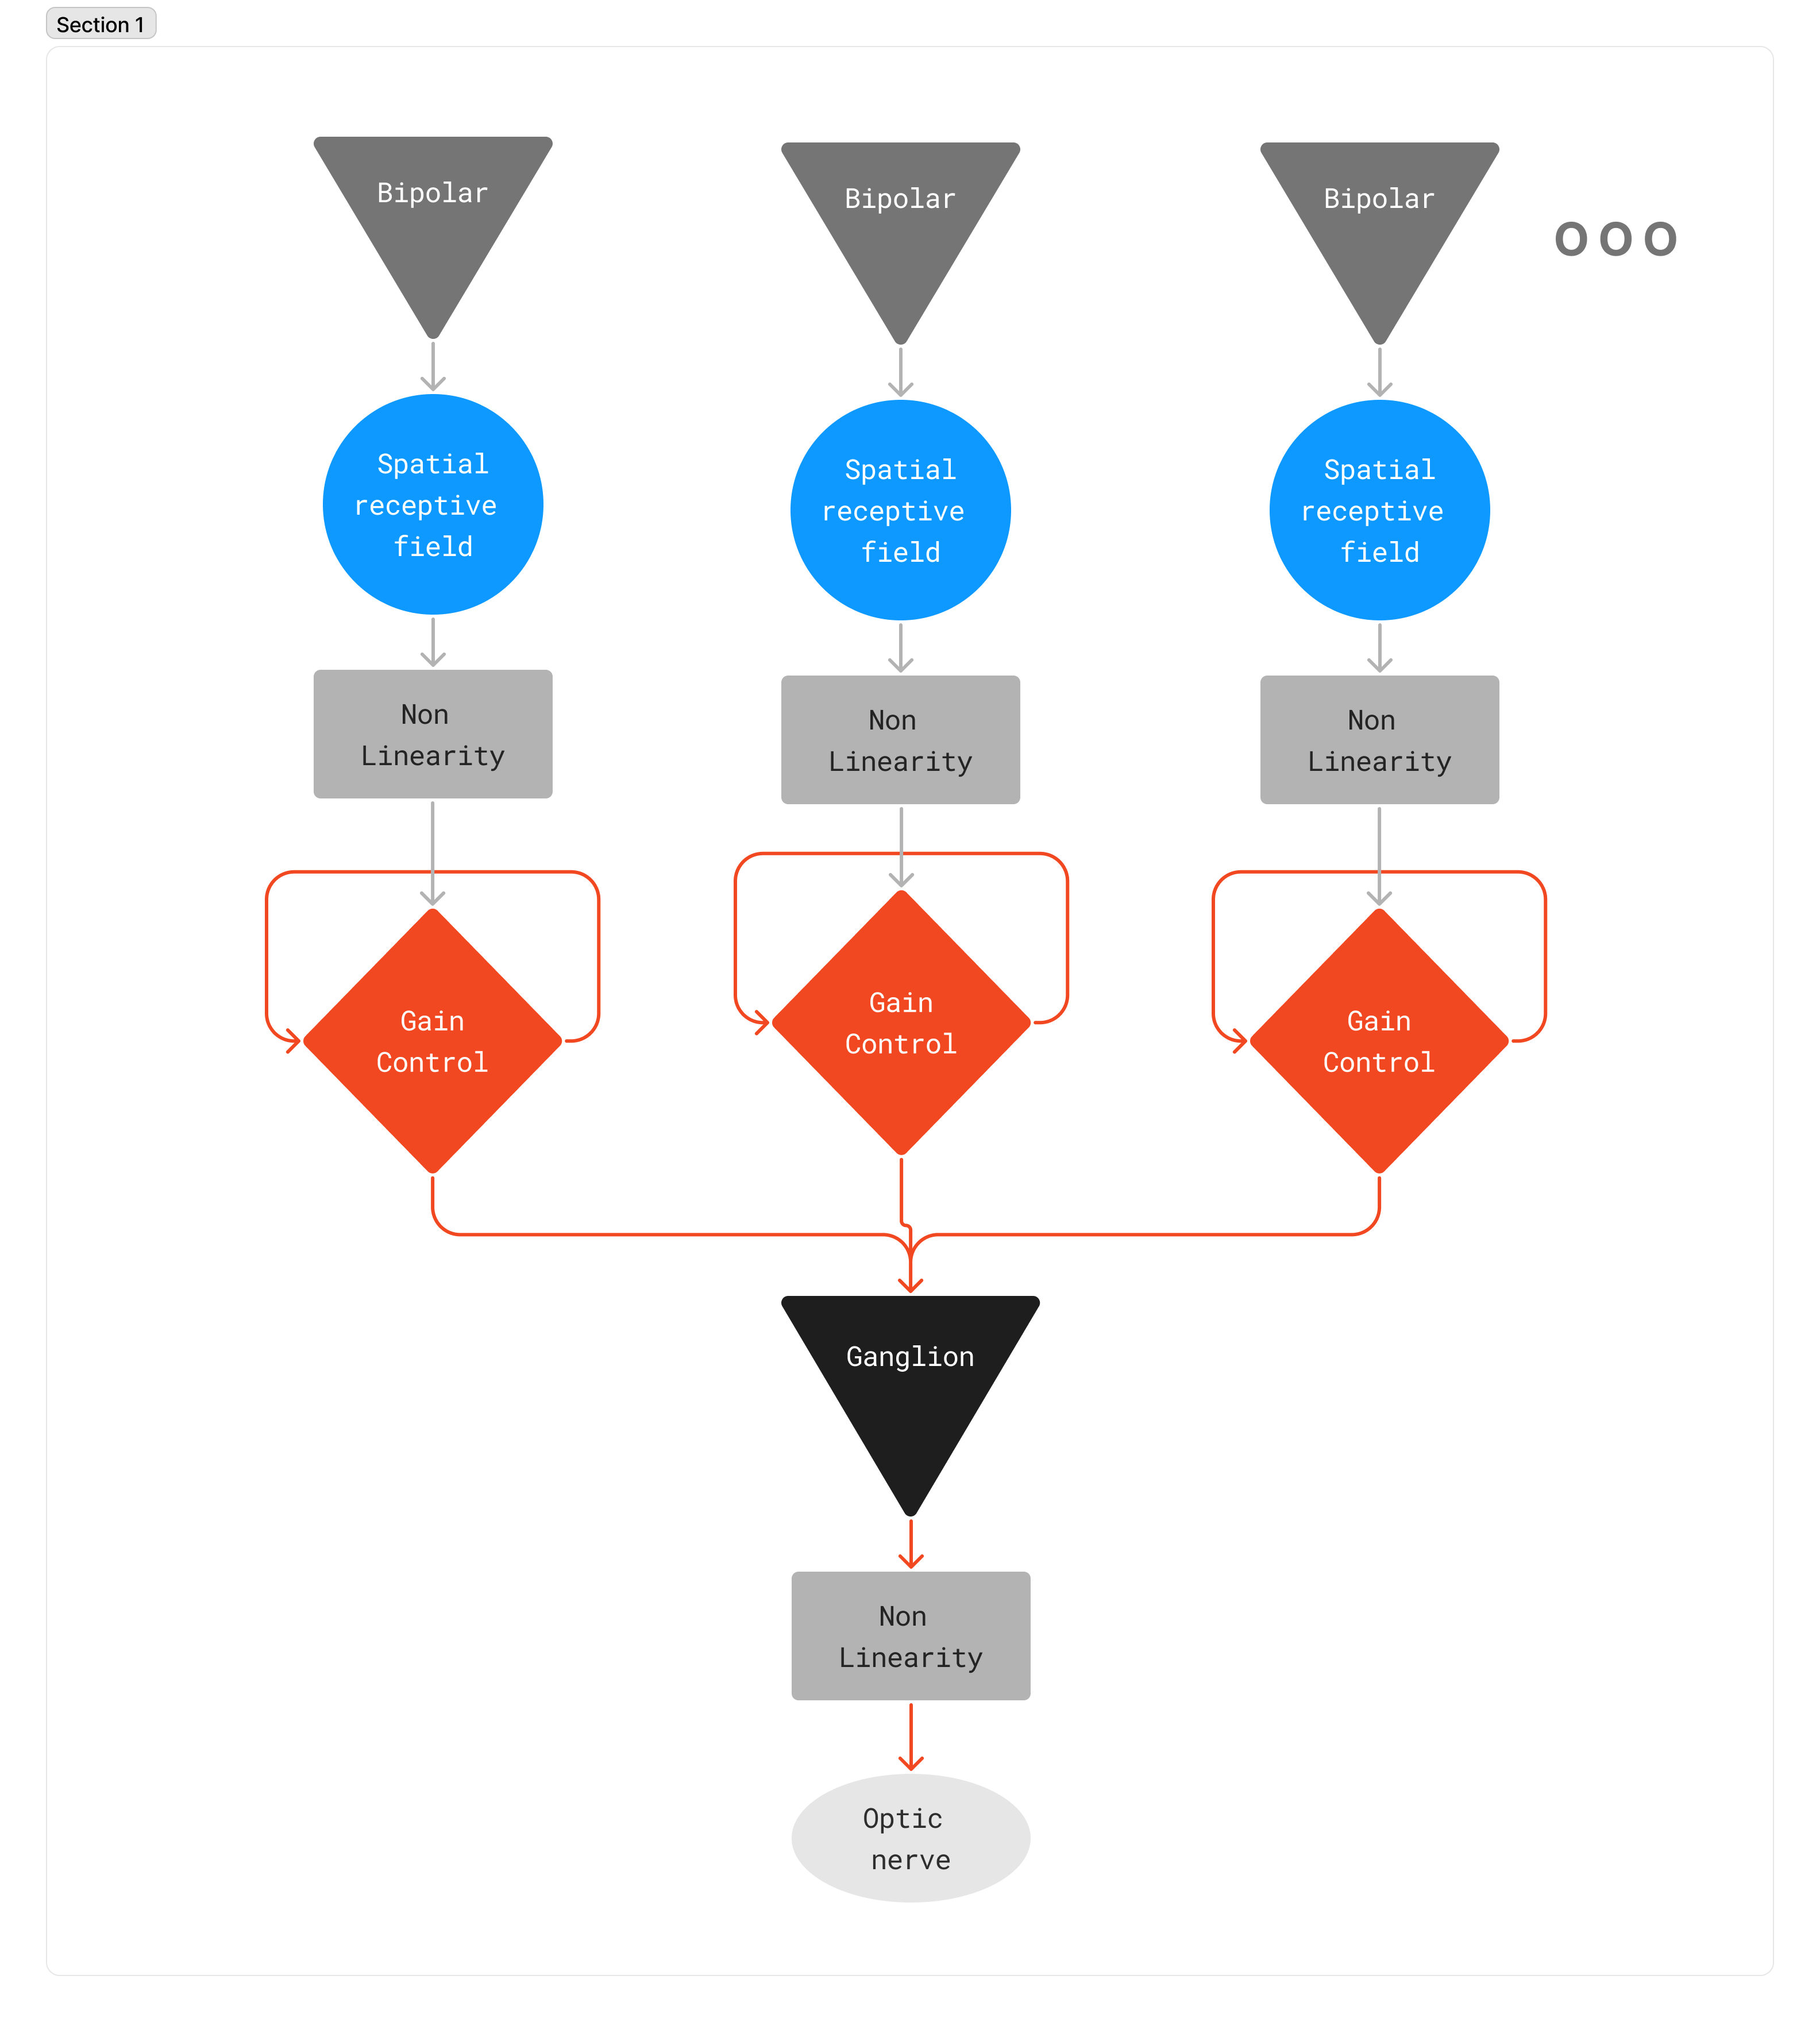
\includegraphics[scale = 0.2]{pics/GCModelDiagram.png}
    \caption{\textbf{Quick sketch of a gain control LNLN model.} Each bipolar
        cell is composed of a linear spatial filter that selectively respond to
        a part
        of the scene, a non-linear activation function, and a gain control
        mechanism
        that scale its output depending on past events. They all converge into
        on
        bipolar cell (forming its receptive field) of which output is also
        modeled
        using a non-linear function.}\label{fig:LNLN}
\end{figure}
We will first study our models in a data agnostic manner and study its behavior
for different set of parameters. We will then fit it on our own experimental
data using an efficient optimization framework in python using strategies
developed in the field of machine learning.